\documentclass{article}
\usepackage[utf8]{inputenc}
\usepackage{graphicx}
\usepackage{listings}
\usepackage{sectsty}
\title{CIS 419/519 Introduction to Machine Learning\newline Assignment 1}
\author{Kuan-Cheng Chiu}
\date{}

\usepackage{listings}
\usepackage{color}

\allsectionsfont{\Large}
\nohang

\definecolor{codegreen}{rgb}{0,0.6,0}
\definecolor{codegray}{rgb}{0.5,0.5,0.5}
\definecolor{codepurple}{rgb}{0.58,0,0.82}
\definecolor{backcolour}{rgb}{0.95,0.95,0.92}

\lstdefinestyle{mystyle}{
	backgroundcolor=\color{backcolour},   
	commentstyle=\color{codegreen},
	keywordstyle=\color{magenta},
	numberstyle=\tiny\color{codegray},
	stringstyle=\color{codepurple},
	basicstyle=\footnotesize,
	breakatwhitespace=false,         
	breaklines=true,                 
	captionpos=b,                    
	keepspaces=true,                 
	numbers=left,                    
	numbersep=5pt,                  
	showspaces=false,                
	showstringspaces=false,
	showtabs=false,                  
	tabsize=2
}

\lstset{style=mystyle}

\begin{document}
\maketitle
 Hello world!

This is a \textbf{bold} text. This is a \underline{underline}. And this is a \textbf{\textit{composed}} style.

\part*{PART I: PROBLEM SET}

\section{Chapter 1}
\subsection{chapter 1 sub}
Some text for chapter one.

\begin{figure}[tbph]
	\centering
	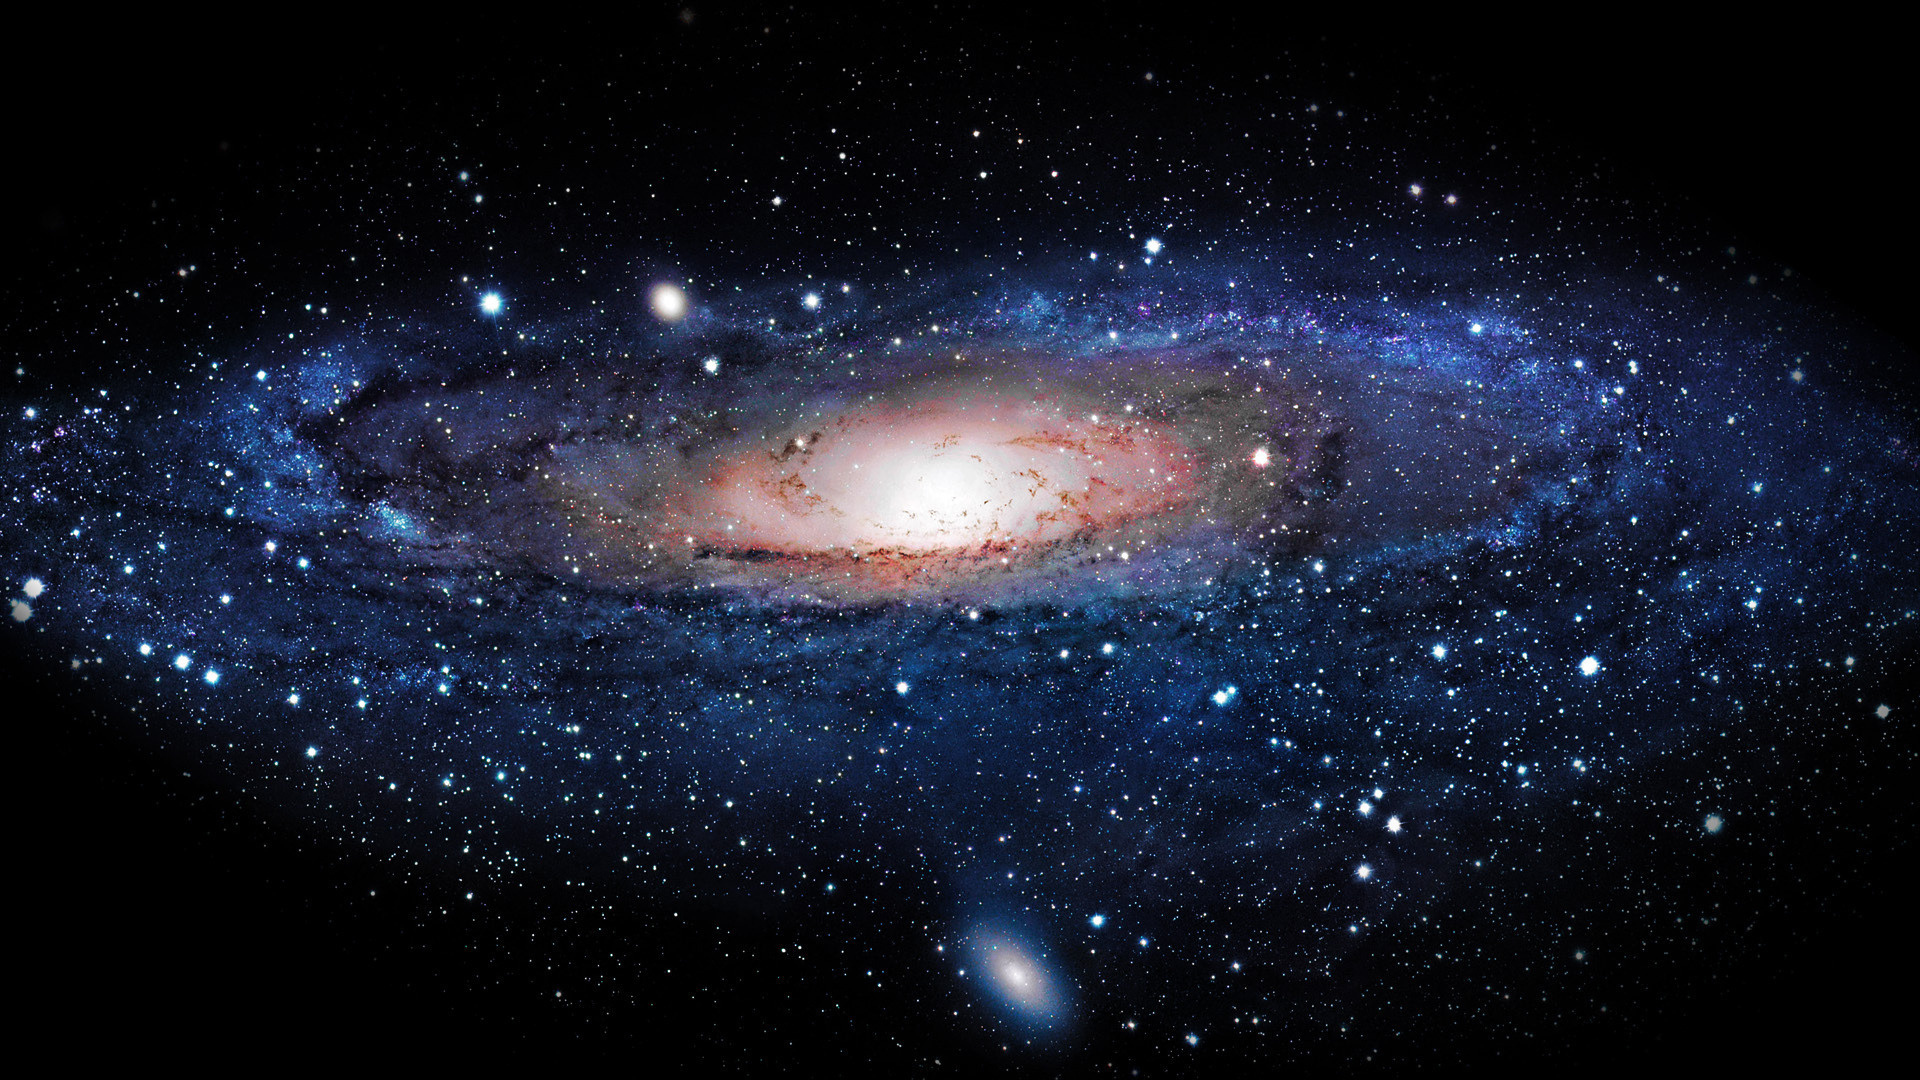
\includegraphics[width=0.8\linewidth]{img}
	\caption{a figure}
	\label{fig:img}
\end{figure}


\section{Chapter 2}

According to Figure~\ref{fig:img}, the space is.

\lstinputlisting[language=Python]{dtree_eval.py}

$A_{x}+1$

\end{document}